\documentclass{article}
\usepackage[utf8]{inputenc}
\usepackage{polski}
\usepackage{graphicx}
\usepackage{natbib}
\usepackage{polski}
\usepackage{tabularx}
\usepackage{wrapfig}
\usepackage{enumitem}
\usepackage{multirow}
\usepackage[left=2cm,right=2cm,vmargin=2.5cm,footnotesep=0.5cm]{geometry}

\title{Technologie informacyjne}
\author{Jakub Jankowiak (258965) }
\date{December 2020}

\begin{document}

\maketitle
\tableofcontents
\clearpage
\section{Co to jest spadek swobodny}
Spadek swobodny jest to fizyczne pojęcie, które w uproszczony sposób opisuje ruch ciała, które na początku znajdowało się w spoczynku i w reakcji na siłę grawitacji zaczęło się poruszać (spadać). Co widać na ilustracji nr.\ref{fig: Obrazek 1}.

\begin{equation}
S=0,5at^2  ,  V=gt , V=\sqrt{2at}
\end{equation}

\section{Przebieg doświadczenia}
Doświadczenie ma na celu zbadanie drogi jaką piłeczka przebędzie w czasie 10s z uwzględnieniem błędu pomiarowego uwzględnionego później na wykresie.
\subsection{Schemat doświadczenia}
\begin{figure}[h]
	\centering
	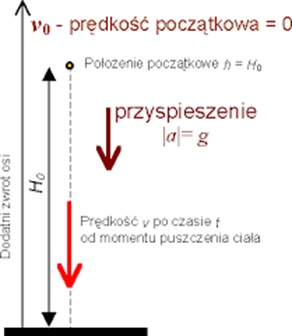
\includegraphics[scale=1.2]{1.1.jpg}
	\caption{Obrazek 1}
	\label{fig: Obrazek 1}
\end{figure}


\newpage
\subsection{Przyrządy pomiarowe}
To przeprowadzenia eksperymenty bądą nam potrzebna Taśma metryczna i Stoper.
\begin{figure}[h]
  \centering
  \begin{minipage}[b]{0.4\textwidth}
    \includegraphics[width=\textwidth]{Taśma.png}
    \caption{Taśma metryczna}
  \end{minipage}
  \hfill
  \begin{minipage}[b]{0.4\textwidth}
    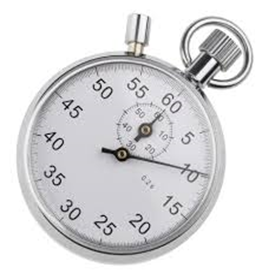
\includegraphics[width=\textwidth]{Stoper.png}
    \caption{Stoper}
  \end{minipage}
\end{figure}

\subsection{Tabele pomiarowe}

\begin{tabular}{|p{4cm}|p{4cm}|}
\hline
\multicolumn{2}{|c|}{Górna część tabeli}\\ \hline
t(s) & s(cm)\\ \hline
0 &	0 \\ \hline
0,1	& -0,035964991\\ \hline
0,2 & 0,128994883\\ \hline
0,3 & 0,525649473\\ \hline
0,4 &	0,788398483\\ \hline
0,5 & 1,080978313 \\ \hline
0,6	& 1,917913767\\ \hline
0,7 &	2,456474829 \\ \hline
0,8 &	3,161508174\\ \hline
0,9 &	4,077312267\\ \hline
1 &	4,820319632\\ \hline
1,1 &	6,183613711\\ \hline
1,2 &	7,294072219\\ \hline
1,3 &	8,466073009\\ \hline
1,4 &	9,856879431\\ \hline
1,5 &	11,31033859\\ \hline
1,6 &	12,82852305\\ \hline
1,7 &	14,38880726\\ \hline
1,8	&   16,17875203\\ \hline
1,9	&   18,09597296\\ \hline
2 & 	20,0671145\\ \hline
\end{tabular}
\quad
\begin{tabular}{|p{4cm}|p{4cm}|}
\hline
\multicolumn{2}{|c|}{Dolna część tabeli}\\ \hline
t(s) & s(cm)\\ \hline
8 &	320,0112379\\ \hline
8,1	& 328,1595394\\ \hline
8,2 &	336,0984231\\ \hline
8,3 &	344,4325829\\ \hline
8,4 &	352,91757\\ \hline
8,5 &	361,2093282\\ \hline
8,6 &	369,8506683\\ \hline
8,7 &	378,4758649\\ \hline
8,8 &	387,0433087\\ \hline
8,9 &	396,1539263\\ \hline
9 &	404,7771388\\ \hline
9,1 &	414,0942262\\ \hline
9,2 &	423,1967377\\ \hline
9,3 &	432,4021378\\ \hline
9,4 &	441,7464959\\ \hline
9,5 &	451,4134528\\ \hline
9,6 &	460,7921066\\ \hline
9,7 &	470,5557483\\ \hline
9,8 &	480,1537412\\ \hline
9,9 & 	489,9402617\\ \hline
10 & 	499,9582302\\ \hline
\end{tabular}

\clearpage
\subsection{Wykres s(t) błędu pomiarowego}

\begin{figure}[h]
	\centering
	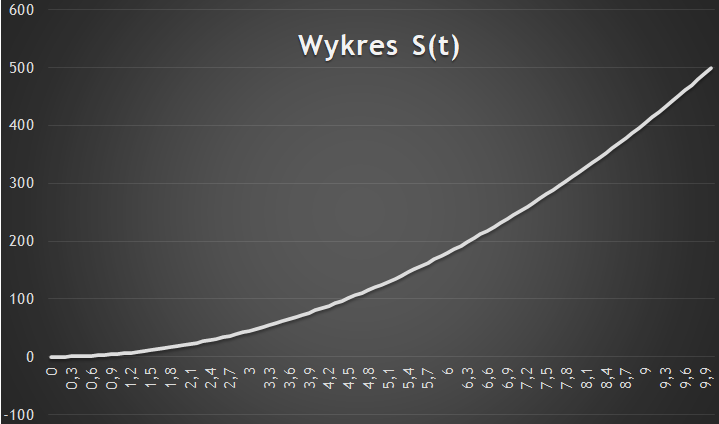
\includegraphics[scale=1.2]{wykres.png}
	\caption{Wykres s(t) błędu pomiarowego}
	\label{fig: Obrazek 1}
\end{figure}

\section{Wnioski}
\begin{itemize}
  \item Przyspieszenie w modelu jest stałe
  \item Prędkość ciała rośnie (oczywiście patrząc tylko do momentu upadku)
  \item Ruch spadających ciał jest jednostajnie przyspieszony
\end{itemize}
\end{document}
